\chapter{Introspective Analysis}
\label{chapter:introspective}
\epigraph{Do what I do. Hold tight and pretend it’s a plan!}{\textit{The 11th Doctor} - Doctor Who}
%\epigraph{The problem with introspection is that it has no end.}{\textit{Philip K. Dick}}

Previous chapters already presented \emph{context-sensitivity} as a common way of pursuing precision and scalability in points-to analysis. An oft-remarked fact about context-sensitivity, however, is that even the best algorithms have a common failure mode when they cannot maintain precision. Past literature reports that ``the performance of a deep-context analysis is bimodal'' \cite{popl:2011:Smaragdakis}; ``context-sensitive analyses have been associated with very large numbers of contexts'' \cite{cc:2006:Lhotak}; ``algorithms completely hit a wall after a few iterations, with the number of tuples exploding exponentially''~\cite{pldi:2011:Liang}. The experimental results in chapter~\ref{chapter:hybrid} (Tables~\ref{tab:hybrid:results-a}-\ref{tab:hybrid:results-b}) show a failure to run a 2-object-sensitive analysis in under 90mins for 2 of 10 DaCapo benchmarks, while 2 more benchmarks take more than 1,000sec, although most other benchmarks of similar or larger size get analyzed in under 200sec.

Thus, when context-sensitivity works, it works formidably, in terms of both precision and performance. When it fails, however, it fails miserably, quickly exploding in complexity. In contrast, context-insensitive analyses uniformly scale well, for the same inputs. Figure~\ref{fig:introspect:intro} vividly demonstrates this phenomenon for the DaCapo benchmarks, analyzed with the \doop{} framework~\cite{oopsla:2009:Bravenboer} under a context-insensitive (insens) analysis and a 2-object-sensitive analysis with a context-sensitive heap (2objH). (The chart truncates the analysis time of the longest-running benchmarks. Two of them, hsqldb and jython, timed out after 90mins on a 24GB machine, and would not terminate even for much longer timeouts.) As can be seen, context-insensitive analyses vary relatively little in performance, while context-sensitivity often causes running time (and memory use) to explode.

\begin{figure}[hp]
\begin{center}
\hspace{-2mm}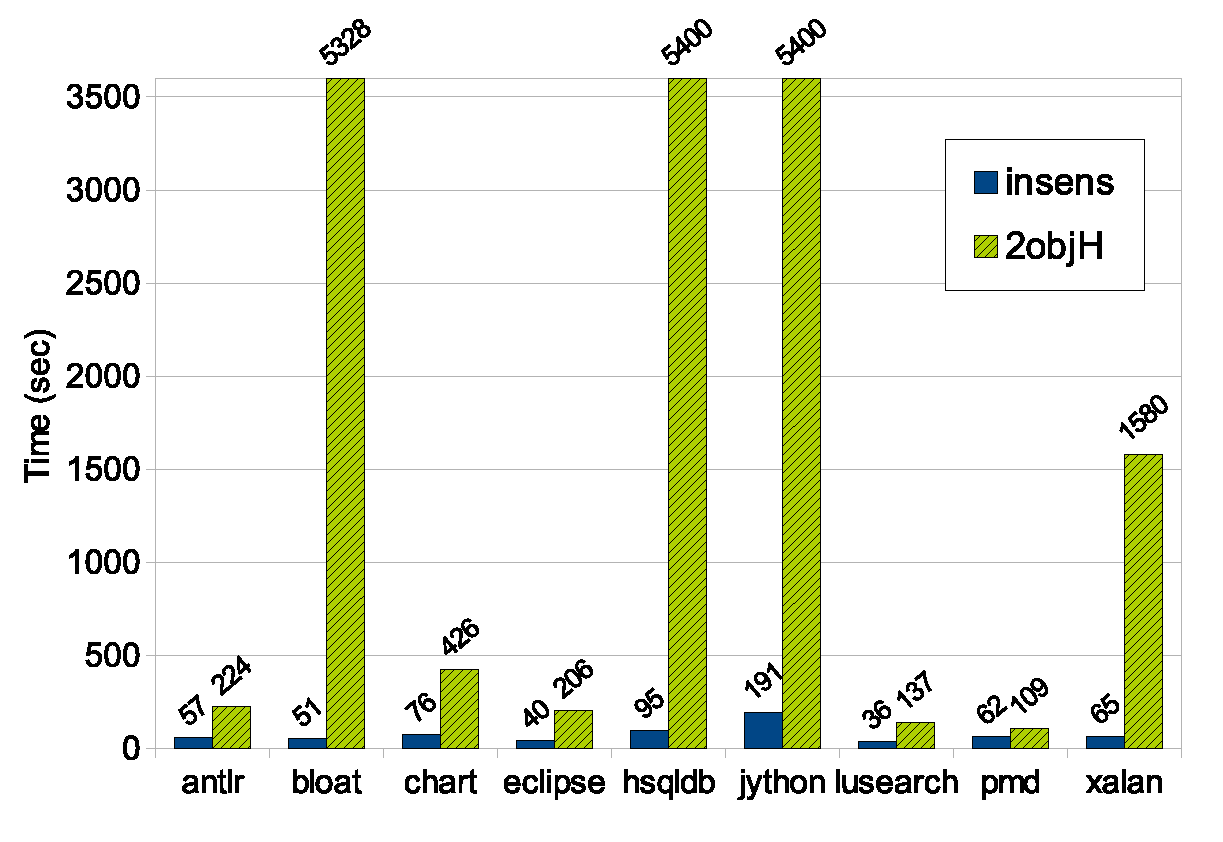
\includegraphics[scale=0.42]{assets/introspective/intro-chart.pdf}
\end{center}
\vspace{-0.6cm}
\caption{Comparison of running times of context-insensitive analysis vs. 2-object-sensitive with context-sensitive heap. The y-axis is truncated to 1hr for readability.}
\label{fig:introspect:intro}
\end{figure}

Faced with this unpredictability of context-sensitivity, a common reaction is to avoid it, favoring context-insensitive analyses, and, consequently, missing significant precision benefits for well-behaved programs. Even worse, for some applications, eschewing expensive context-sensitivity is not an option---a context-insensitive analysis is just not good enough and even an often inexpensive context-sensitive analysis (e.g., 2-type-sensitive with a context-sensitive heap) fails to yield good precision. Reports from industry~\cite{misc:Cifuentes} and academic researchers~\cite{misc:Chong} alike reiterate that precise context-sensitivity is essential for information-flow analysis, taint analysis, and other security analyses.

We can ask ourselves, why does this scalability barrier arise? The core problem is that, for some objects or methods, the points-to information is imprecise enough that more context does not help, while incurring a heavy overhead \cite{popl:2011:Smaragdakis}. Consider a method argument that was found to point to $n$ objects by a less precise analysis. Further analyzing the method in $c$ different contexts (or, equivalently, increasing context depth by 1) will ideally yield $n/c$ points-to facts per context, perfectly splitting the previous $n$-object points-to set, thus yielding both precision and scalability. In the worst case, however, increasing the context depth will result in $c$ copies of $n$ points-to facts each: the extra context depth will not have yielded more precision, but will have multiplied the space and time costs. When this occurs, the analysis cost explodes for greater context depths.

The focus of this chapter is on the detection and prevention of pathological behavior in context-sensitive analyses, with minimal intervention. In this way, we achieve many of the precision benefits of context-sensitivity without sacrificing scalability. It does not seem possible to know in advance (e.g., by identifying syntactic features of the program) which program elements may be responsible for pathological behavior. Nevertheless, we argue that it is possible to identify such elements with a scalable context-insensitive analysis. We introduce the concept of \emph{introspective context-sensitivity}: during a first, context-insensitive, analysis pass, the analysis observes symptoms indicating that the cost may get out of hand for deeper context. This detects exactly the pathology identified above. In its simplest form, the analysis will ask ``which program sites currently have points-to information that may grow too large for an extra level of context?'' Using a configurable second pass\footnote{In theory, this pattern could be repeated for more passes.}, such sites will be re-analyzed with shallow context, even though the rest of the program will be re-analyzed with a deeper context.

In intuitive terms, introspective context-sensitivity performs a cost-benefit calculation, with an emphasis on the potential cost of increasing context depth, since cost can be estimated more reliably. Fairly simple---yet not always obvious---heuristics can estimate this cost well. 

As a general pattern, this approach is familiar. Even in the context of points-to analysis, the pattern of performing a coarse-grained analysis and using it to tune a finer-grained one has been explored before, as in earlier \emph{refinement-based}~\cite{pldi:2006:Sridharan} or \emph{pruning}~\cite{pldi:2011:Liang} techniques. Nevertheless, such past approaches differ from our approach in terms of both external applicability and impact: they fundamentally apply to demand-driven (as opposed to all-points on the entire program) analyses and they either do not target context depth or only apply to specific kinds of context---related work in Section~\ref{sec:related:introspective} includes a detailed discussion.

The net outcome of our work is not a ``first line of defense'' analysis, but an ``if all else fails'' analysis. Users are still better advised to first use traditional context-sensitive algorithms, in the hope that these will scale well and provide good precision. When this fails, however, we show that we can provide a highly reliable knob for filtering out worst-case performance at a small cost in precision. Our experiments demonstrate that the user can ``dial-in'' scalability, to the exact level required. For instance, as seen in Figure~\ref{fig:introspect:intro}, a precise 2objH analysis fails to run in under 90mins on a 24GB machine for 3 of our experimental subjects. However, we can get an introspective context-sensitive analysis to scale to all benchmarks in under 12mins, while still gaining significant precision over a context-insensitive analysis. Yet another introspective analysis scales to all but one benchmark in under 20mins, while sacrificing a fraction of precision (keeping about 2/3 of the precision gains of a full 2objH analysis). For call-site sensitive analyses, the gains are even more pronounced, with several benchmarks exhibiting at least 300\% speedups, without sacrificing nearly any precision.

Overall, this chapter describes the following contributions:

\begin{itemize}
\item We offer an approach to refining a context-sensitive analysis while avoiding its worst-case cost. The approach relies on first running a context-insensitive analysis and using its results to inform the application of context-sensitivity. Much of the challenge concerns the question of \emph{how} to use this information, i.e.,  what heuristics yield good behavior.

\item We encode the approach in a simple form, by incremental modifications of a general declarative analysis pattern. Therefore, our approach works on virtually any algorithm expressed in this manner. Our implementation is on the \doop{} framework and already applies to the over 30 analysis algorithms that the framework has to offer.

\item We show experimentally the benefit of introspective context-sensitivity. We quantify the precision loss and scalability gains for different parameter settings and show that there is a dial that users can tune, to select points in this spectrum. Even our high-precision settings are effective in eliminating behavior outliers, showing that introspective context-sensitivity has core value: previously hopeless analyses suddenly become feasible, for little precision loss. We believe that the result is to give confidence that context-sensitive analyses can be used in virtually any setting and not just in the nebulous ``when they work well'' case.
\end{itemize}

\section{Formulation of Introspective Context-Sensitivity}
\label{sec:introspect:model}

We demonstrate introspective context-sensitivity via incremental changes to the existing model for context-sensitive, flow-insensitive points-to analysis algorithms presented in Section~\ref{sec:back:model}. As previously mentioned, the logical formalism of this model is very close to the core components of our actual analysis implementation.

\paragraphhead{Input relations.}
Two additional input relations are added to those presented in Figure~\ref{fig:back:input} and are used exclusively for the purposes of introspective context-sensitivity. \relname{SiteToRefine} and \relname{ObjectToRefine} encode the program points (invocation site/method combinations, and allocation sites) that will employ a different context abstraction from the rest.

\begin{figure}[hb]
\begin{datalog}
\rel{SiteToRefine}{invo: I, meth: M} \\ 
\rel{ObjectToRefine}{heap: H}
\end{datalog}
\caption[]{Additional input Datalog relations expanding those of Figure~\ref{fig:back:input}.}
\label{fig:introspect:input}
\end{figure}

\paragraphhead{Computed (output) relations.}
No additional output relations need to be added to those of Figure~\ref{fig:back:output}.

\paragraphhead{Constructors for context-sensitivity.}
As previously mentioned, the base rules of any analysis are not concerned with what kind of context-sensitivity is used. The context flavor and depth aspects are completely hidden mainly behind constructor functions \consname{Record} and \consname{Merge}. These functions are sufficient for modeling a very large variety of context-sensitive analyses. In addition to those two, introspective context-sensitivity adds two more constructor functions to act as counterparts---\consname{RecordRefined} and \consname{MergeRefined}. They are directly analogous to \consname{Record} and \consname{Merge} but just apply to different program points. These constructors are the machinery for introspective context-sensitivity: they vary the context-sensitivity of the analysis for a subset of the heap objects and methods.

\begin{figure}[htp]
\begin{datalog}
\cons{RecordRefined}{heap: H, ctx: C}{newHCtx: HC} \\
\cons{MergeRefined}{heap: H, hctx: HC, invo: I, ctx: C}{newCtx: C}
\end{datalog}
\caption[]{Additional constructors of contexts that filter which objects and which call-sites/target methods should have a different (i.e., more precise) context in introspective context-sensitivity.}
\label{fig:introspect:output}
\end{figure}

\paragraphhead{Analysis logic.}
The rules for introspective context-sensitivity supplement the existing logic presented in Section~\ref{sec:back:model}. Out of the core nine rules, only two need to be enhanced with duplicate versions, as shown in Figure~\ref{fig:introspect:rules}. Each rule pair offers a version for the default handling of context and another for the more precise handling. (In the full implementation, there are some two-dozen rules that construct new contexts, instead of the two in the model, and all are duplicated accordingly.)

The first pair considers the handling of object allocation, with the first rule applying when the allocation is to be treated with no additional precision, whereas the second applies a more refined context---whether the \relname{ObjectToRefine} holds or not for the current allocation site. The different handling of context is controlled via the \consname{Record} and \consname{RecordRefined} functions, respectively.

The second pair is somewhat more involved but still follows the same reasoning, applied to method invocations. The filtering is controlled via the \relname{SiteToRefine} relation and the different handling of (calling) context is done via the \consname{Merge} and \consname{MergeRefined} functions.

Therefore, we can effect any change we want to the context-sensitivity of an analysis, on a per-object/per-call-site basis, by supplying the right input relations \relname{ObjectToRefine} or \relname{SiteToRefine} and setting the appropriate constructors, \consname{RecordRefined} and \consname{MergeRefined} to implement a different flavor/depth of context-sensitivity. We discuss such options next.

\begin{figure}[h!tp]
\begin{datalog}
\cons{Record}{heap, ctx}{?hctx}, \\
\commrel{VarPointsTo}{var, ctx, heap, ?hctx} \dlIf{} \\
    \commrel{Reachable}{meth, ctx}, \commrel{Alloc}{var, heap, meth}, \\
    ! \rel{ObjectToRefine}{heap}. \\
\\
\comm{// Duplicate rule, for introspective context-sensitivity} \\
\cons{RecordRefined}{heap, ctx}{?hctx}, \\
\commrel{VarPointsTo}{var, ctx, heap, ?hctx} \dlIf{} \\
    \commrel{Reachable}{meth, ctx}, \commrel{Alloc}{var, heap, meth}, \\
    \rel{ObjectToRefine}{heap}. \\
%
\noindent\rule{\textwidth}{0.5pt}\\
%
\cons{Merge}{heap, hctx, invo, callerCtx}{?calleeCtx}, \\
\commrel{Reachable}{toMeth, ?calleeCtx}, \\
\commrel{VarPointsTo}{this, ?calleeCtx, heap, hctx}, \\
\commrel{CallGraphEdge}{invo, callerCtx, toMeth, ?calleeCtx} \dlIf{} \\
    \commrel{VCall}{base, sig, invo, inMeth}, \\
    \commrel{Reachable}{inMeth, callerCtx}, \\
    \commrel{VarPointsTo}{base, callerCtx, heap, hctx},\\
    \commrel{HeapType}{heap, heapT}, \\
    \commrel{Lookup}{heapT, sig, toMeth},\\
    \commrel{ThisVar}{toMeth, this}, \\
    ! \rel{SiteToRefine}{invo, toMeth}. \\
\\
\comm{// Duplicate rule, for introspective context-sensitivity} \\
\cons{MergeRefined}{heap, hctx, invo, callerCtx}{?calleeCtx}, \\
\commrel{Reachable}{toMeth, ?calleeCtx}, \\
\commrel{VarPointsTo}{this, ?calleeCtx, heap, hctx}, \\
\commrel{CallGraphEdge}{invo, callerCtx, toMeth, ?calleeCtx} \dlIf{} \\
    \commrel{VCall}{base, sig, invo, inMeth}, \\
    \commrel{Reachable}{inMeth, callerCtx}, \\
    \commrel{VarPointsTo}{base, callerCtx, heap, hctx},\\
    \commrel{HeapType}{heap, heapT}, \\
    \commrel{Lookup}{heapT, sig, toMeth},\\
    \commrel{ThisVar}{toMeth, this}, \\
    \rel{SiteToRefine}{invo, toMeth}.
\end{datalog}
\caption[]{Datalog rules for different handling of context creation on a per-object/per-call-site basis.}
\label{fig:introspect:rules}
\end{figure}


\section{How To Selectively Refine}
\label{sec:introspect:heuristics}

The model of the previous section allows to easily configure context-sensitivity in a large variety of ways. For instance, some methods (or some call-sites) can be analyzed with object-sensitivity while others are analyzed with call-site sensitivity, of any depth. One aspect to determine, therefore, is the two analyses that will be used in different program points.

Another question is how to populate the \relname{ObjectToRefine} and \relname{SiteToRefine} input relations. One could attempt to do so by mere syntactic inspection of the program. For example, methods containing cast statements can be analyzed with a higher context depth. In our work, we have failed to identify such syntactic heuristics that would yield benefit.

Instead, our introspective context-sensitivity consists of running the analysis \emph{twice}. The first time, \relname{ObjectToRefine} and \relname{SiteToRefine} are \emph{empty} and the \consname{Merge}/\consname{Record} context constructors are set so that an inexpensive but scalable analysis is performed. In our experimental setting, these constuctor functions return a unique constant value, \args{$\star$}, resulting in a context-insensitive analysis:

\begin{quote}
\cons{Record}{heap,ctx}{$\star$}\\
\cons{Merge}{heap, hctx, invo, ctx}{$\star$} \\
\end{quote}

The \consname{MergeRefined} and \consname{RecordRefined} constructors are set to implement an expensive context-sensitive analysis, following the techniques of Chapter~\ref{chapter:hybrid}. Yet, these constructors are not relevant in the first analysis run, since the rules employing them are predicated on having elements in \relname{SiteToRefine} and \relname{ObjectToRefine}, respectively.

Subsequently, we use the results of the context-insensitive analysis to compute which program elements to refine (i.e., populate the \relname{SiteToRefine} and \relname{ObjectToRefine} relations), and run the analysis a second time. The result is that a subset of the program elements are analyzed context-sensitively, while the rest are analyzed context-insensitively even during the second analysis run. In practical terms, the former set is larger than the latter: we focus on identifying a relatively small number of program elements that may disproportionately affect analysis costs and to analyze them context-insensitively, while the majority of program elements are analyzed context-sensitively.

Therefore, the main challenge is to identify a program client analysis (over the results of a context-insensitive points-to analysis) to predict which program elements should not be refined. Our criterion is based on cost rather than expected benefit, since the latter is very hard to estimate in an all-points (as opposed to demand-driven) program analysis. There are several cost metrics that we can mix-and-match to create introspective analysis heuristics:

\begin{enumerate}
\item \label{metric-arginflow} Compute at every invocation site the cumulative size of all points-to sets of actual arguments to the method call. (This is the argument \emph{in-flow} of the method call.)

\item \label{metric-methvpt} Compute for every method the cumulative (or maximum, for a variant of the metric) size of points-to sets over all local variables. (This is the method's \emph{total points-to volume} or \emph{max var-points-to}.)

\item \label{metric-maxfield} Compute for each object (i.e., allocation site) the maximum (or total, for a variant of the metric) field points-to set over all of its fields (This is the object's \emph{max field points-to}, or \emph{total field points-to}.)

\item \label{metric-methodmaxfield} Compute for every method the maximum max field-points-to (metric~\ref{metric-maxfield}) among objects pointed to by the method's local variables. (This is the method's \emph{max var-field points-to}.)

\item \label{metric-pointedby} Compute for each object (i.e., allocation site) the number of local variables pointing to it. (This is the object's \emph{pointed-by} metric.)
\end{enumerate}

As can be seen, these metrics can vary in sophistication but all of them attempt to estimate the cost that will be incurred if the same method or allocation site were to be analyzed context-sensitively. Indeed, our emphasis is not on the sophistication of the metrics or on their fine-tuning. Instead, it is on their simplicity and ease of composition so that one can create parameterizable analyses: a knob for adjusting the precision/scalability tradeoff. For example, we propose two heuristic combinations of these metrics:

\begin{quote}
\paragraphhead{Heuristic-A.}
% tempH heuristic in the initial source code
Refine all allocation sites except those with a \emph{pointed-by} (Metric~\#\ref{metric-pointedby}) higher than a constant $K$.  Refine all method call-sites except those with either an \emph{in-flow} (Metric~\#\ref{metric-arginflow}) higher than a constant $L$ or a \emph{max var-field points-to} (Metric~\#\ref{metric-methodmaxfield}) higher than a constant $M$.
\end{quote}

\begin{quote}
\paragraphhead{Heuristic-B.}
% tempO heuristic in the initial source code
Refine all method call-sites except those that invoke methods with a \emph{total points-to volume} (Metric~\#\ref{metric-methvpt}) above a constant $P$. Refine all object allocations except those for which the product of \emph{total field points-to} and \emph{pointed-by} (Metrics~\#\ref{metric-maxfield} and \#\ref{metric-pointedby}) exceeds a constant $Q$. The product of these two metrics can be seen as an object's total potential for weighing down the analysis.
\end{quote}

These heuristics are themselves tunable, by adjusting the constant parameters. In the rest of the chapter, when we refer to \emph{Heuristic-A} in measurements, the values of $K$, $L$, $M$ will be 100, 100, and 200, respectively; when we refer to \emph{Heuristic-B}, the values of $P$ and $Q$ will both be 10000. The point of picking clear-cut reference numbers is to argue that the value of the technique does not come from excessive tuning but from the underlying power of the introspective analysis idea---even relatively large variations of these numbers make scarcely any difference in the total picture of results over multiple programs.

\paragraph*{Intuition.} 
The main insight behind our Heuristic-Approach is that there are many program elements whose analysis cost is vastly disproportionate to their importance. If such elements are analyzed less precisely, the analysis will avoid significant burden without incurring large precision losses. The above two heuristics try to estimate ``disproportionate cost'' but have no way of estimating the ``importance'' of a program element. It would be an interesting direction for future work to estimate this importance, i.e., to define metrics that capture the extent of the impact of a program element's precision on all other program elements.

Furthermore, a program element with very large cost, in terms of associated points-to facts, may be hopeless for good enough precision anyway. On the other hand, the above intuition could potentially unfold the other way: it is possible that context-sensitivity can productively distinguish seemingly-imprecise program elements (e.g., methods with large cumulative points-to sets, but also many callers) and maintain precision.

\paragraph*{Implementation.}
The above metrics and heuristics can be easily implemented as short analyses over the result of a context-insensitive points-to analysis. For instance, the implementation of the \emph{in-flow} metric (\#\ref{metric-arginflow}) is the following Datalog rules, which define an intermediate predicate and aggregate over it. (``\args{\_}'' is a nameless variable denoting any value, and ``\texttt{\{...\}}'' denotes an aggregate operation over the relations inside the curly brackets ---in our case a total count of matching tuples.)

\begin{figure}[h]
\begin{datalog}
\rel{HeapsPerInvocationPerArg}{invo, arg, heap} \dlIf{} \\
    \rel{CallGraphEdge}{invo, \_, \_, \_},\\
    \rel{ActualArg}{invo, \_, arg},\\
    \rel{VarPointsTo}{arg, \_, heap, \_}.\\
\\
\rel{InFlow}{invo, ?result} \dlIf{} \\
    \aggregate{COUNT}{\rel{HeapsPerInvocationPerArg}{invo, \_, \_}}{?result}.
\end{datalog}
\end{figure}




\section{Evaluation}

Our evaluation setting uses the LogicBlox Datalog engine, v.3.9.0, on a Xeon E5530 2.4GHz machine with only one thread running at a time and 24GB of RAM. We analyze the DaCapo benchmark programs (v.2006-10-MR2) with Open JDK 1.6.0\_24. We run all benchmarks with default \doop{} settings, including full reflection support. We selected a priori 6 of the Dacapo benchmarks as our experimental subjects: these are the programs that exhibit scalability problems based on past literature (e.g., Chapter~\ref{chapter:hybrid}). Other benchmarks typically run in half the time of the fastest benchmark of our set for deep context-sensitive analyses. Since our technique is explicitly not a ``first line of defense'', benchmarks that are already certain to scale are out of scope.

\begin{figure*}[h!tp]
\begin{center}
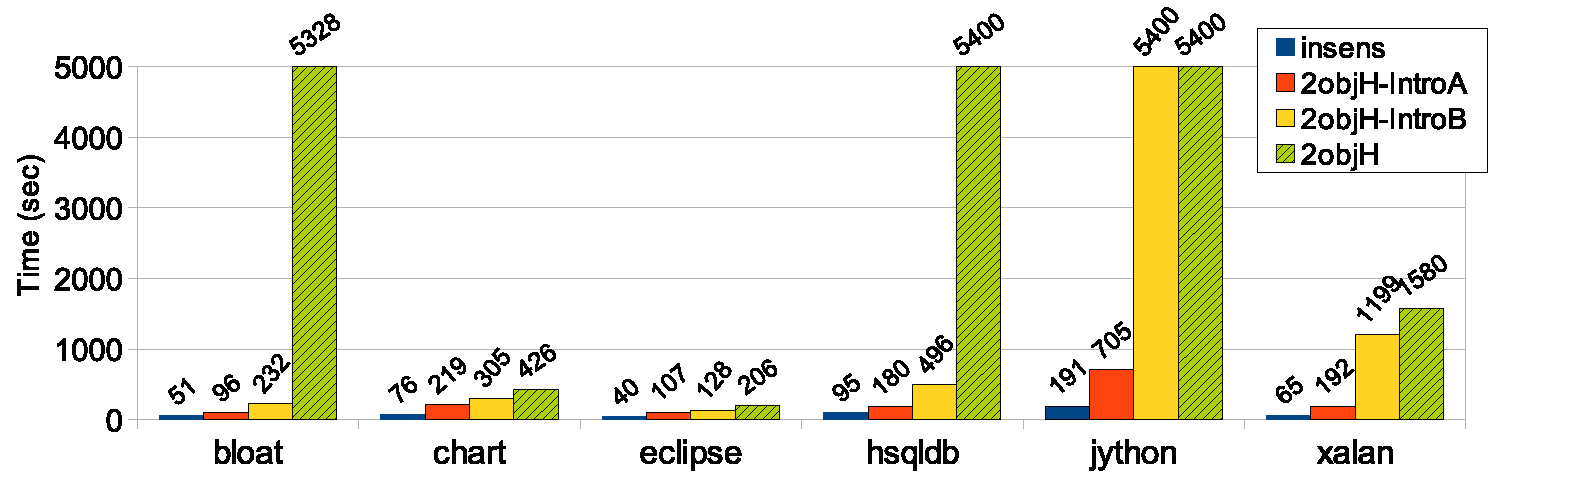
\includegraphics[scale=0.54]{assets/introspective/2objHtime.pdf} \\
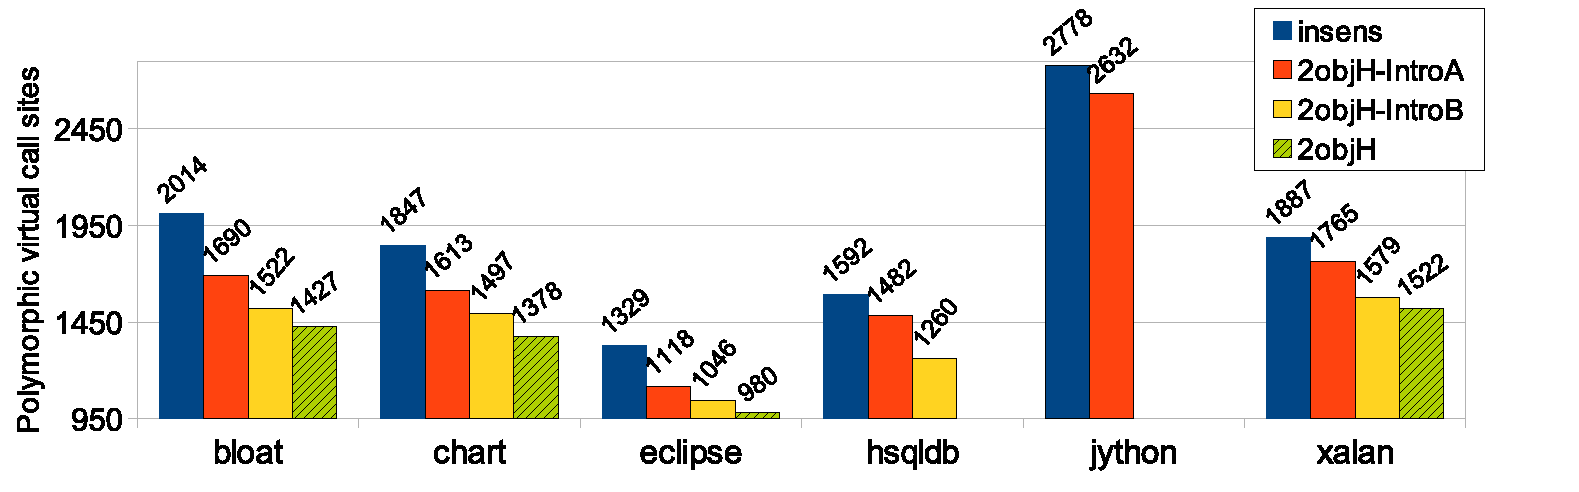
\includegraphics[scale=0.54]{assets/introspective/2objHvcalls.pdf} \\
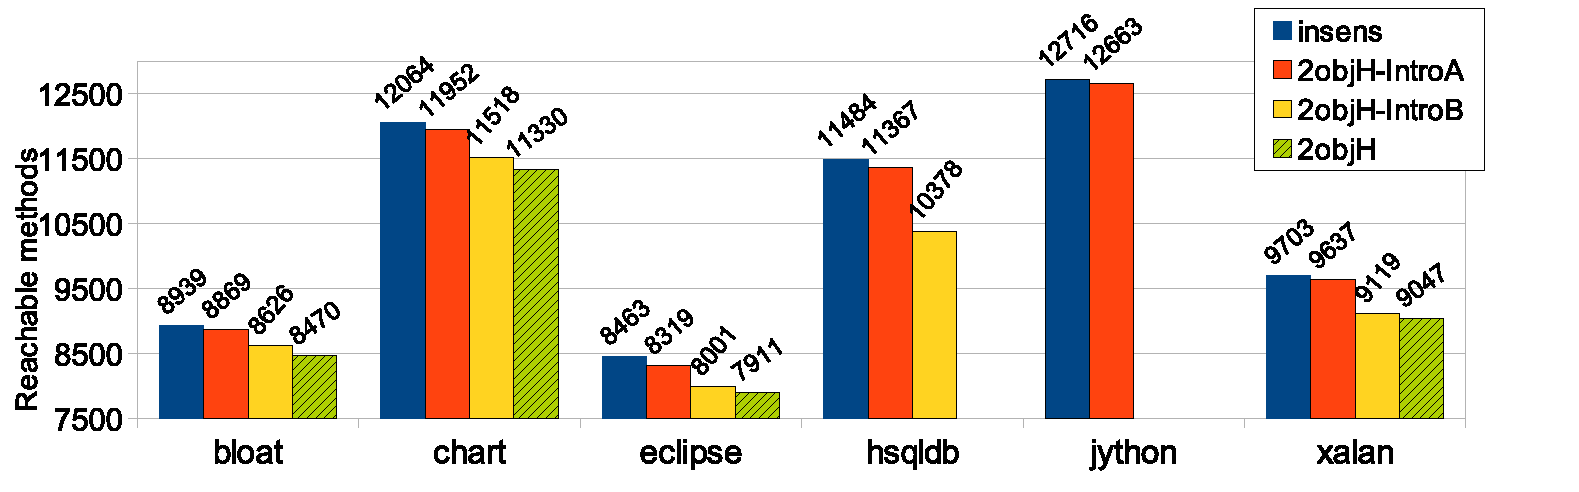
\includegraphics[scale=0.54]{assets/introspective/2objHmeths.pdf} \\
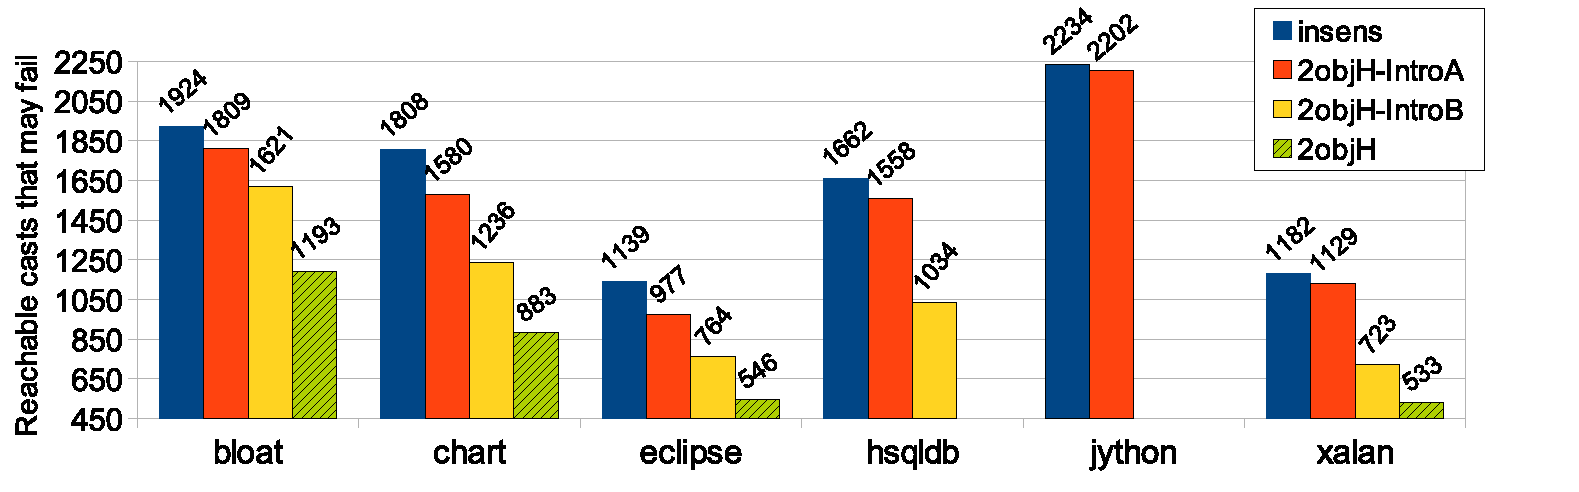
\includegraphics[scale=0.54]{assets/introspective/2objHcasts.pdf}
\end{center}
\caption{Performance and precision (3 separate metrics: calls that cannot be devirtualized, reachable methods, casts that cannot be eliminated) for introspective context-sensitive variants of a \textbf{2objH} analysis, compared with baselines (2objH and insensitive).}
\label{fig:introspect:2objH-chart}
\end{figure*}


\begin{figure*}[h!tp]
\begin{center}
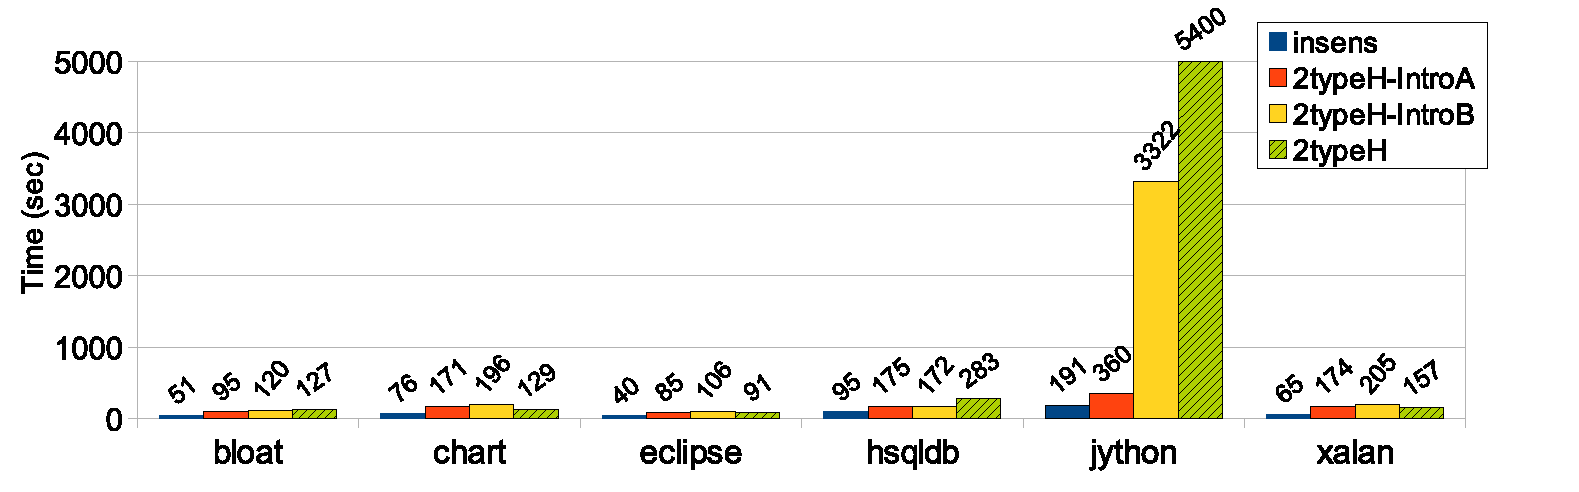
\includegraphics[scale=0.54]{assets/introspective/2typeHtime.pdf} \\
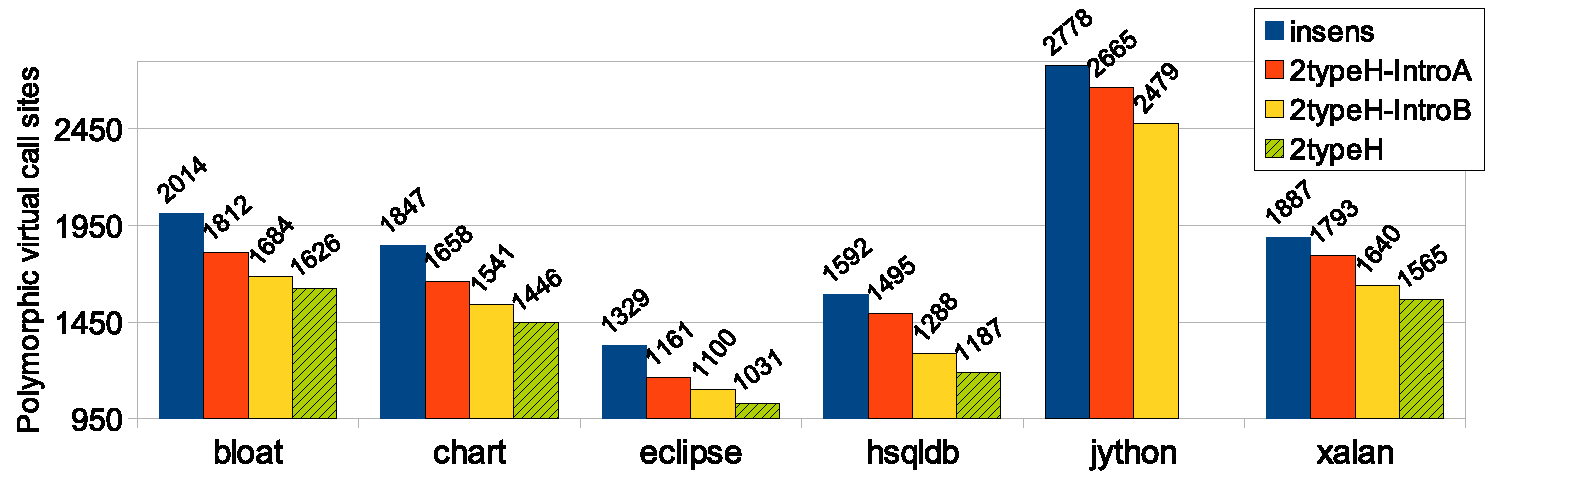
\includegraphics[scale=0.54]{assets/introspective/2typeHvcalls.pdf} \\
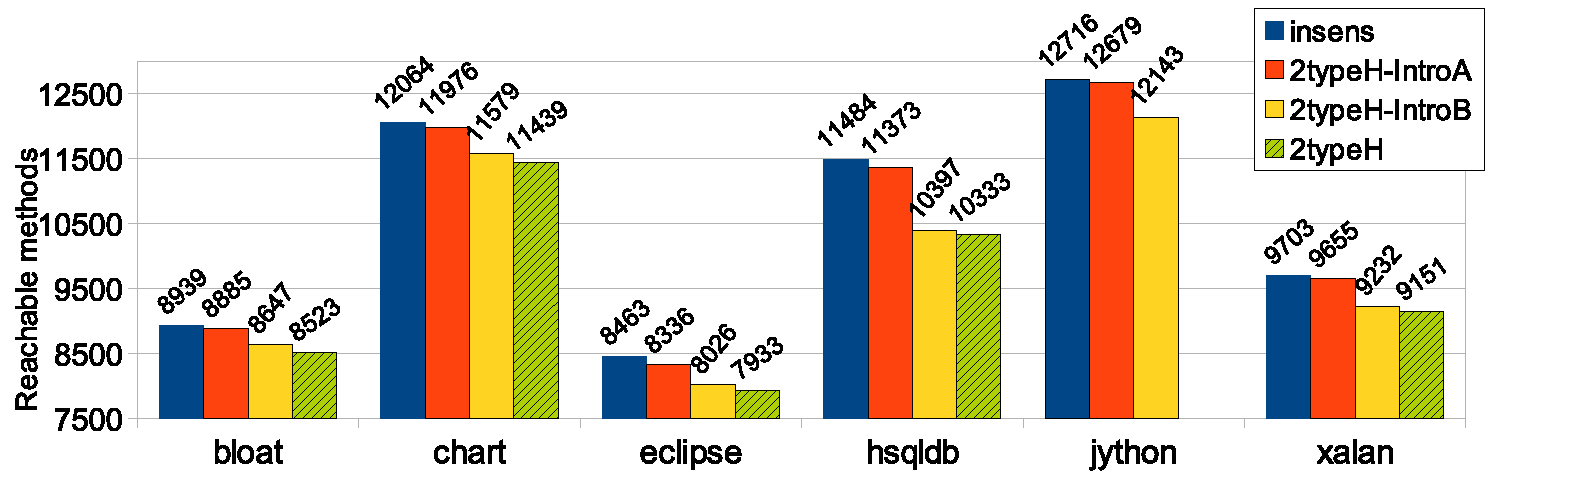
\includegraphics[scale=0.54]{assets/introspective/2typeHmeths.pdf} \\
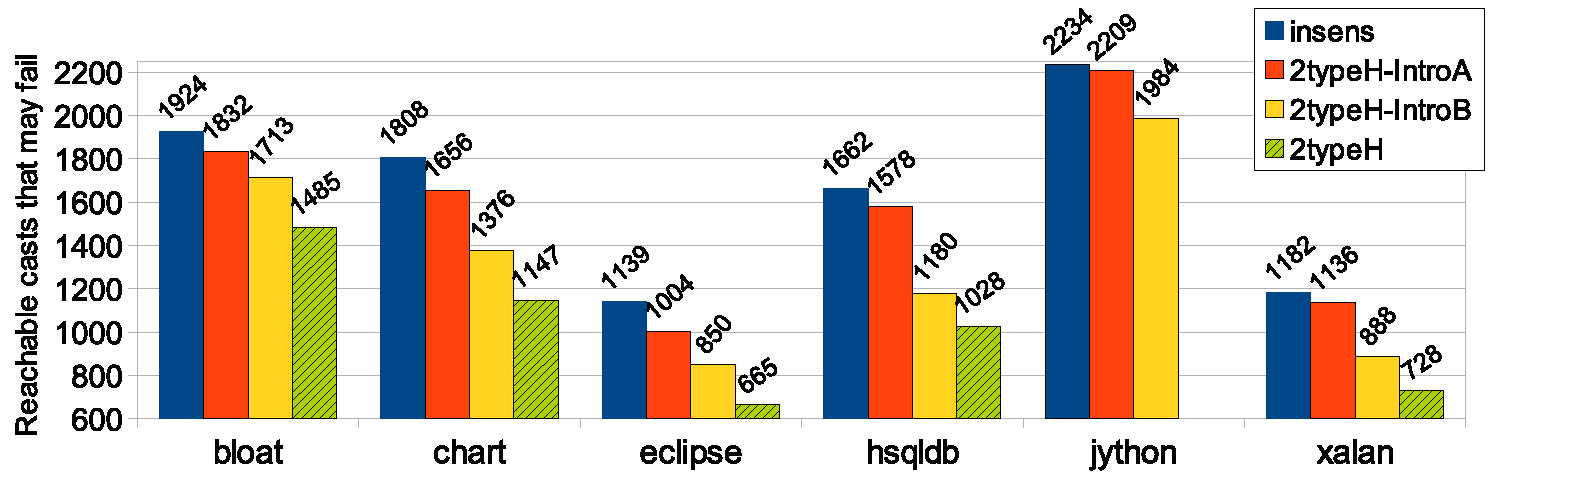
\includegraphics[scale=0.54]{assets/introspective/2typeHcasts.pdf}
\end{center}
\caption{Performance and precision (3 separate metrics: calls that cannot be devirtualized, reachable methods, casts that cannot be eliminated) for introspective context-sensitive variants of a \textbf{2typeH} analysis, compared with baselines (2typeH and insensitive).}
\label{fig:introspect:2typeH-chart}
\end{figure*}


\begin{figure*}[t!bp]
\begin{center}
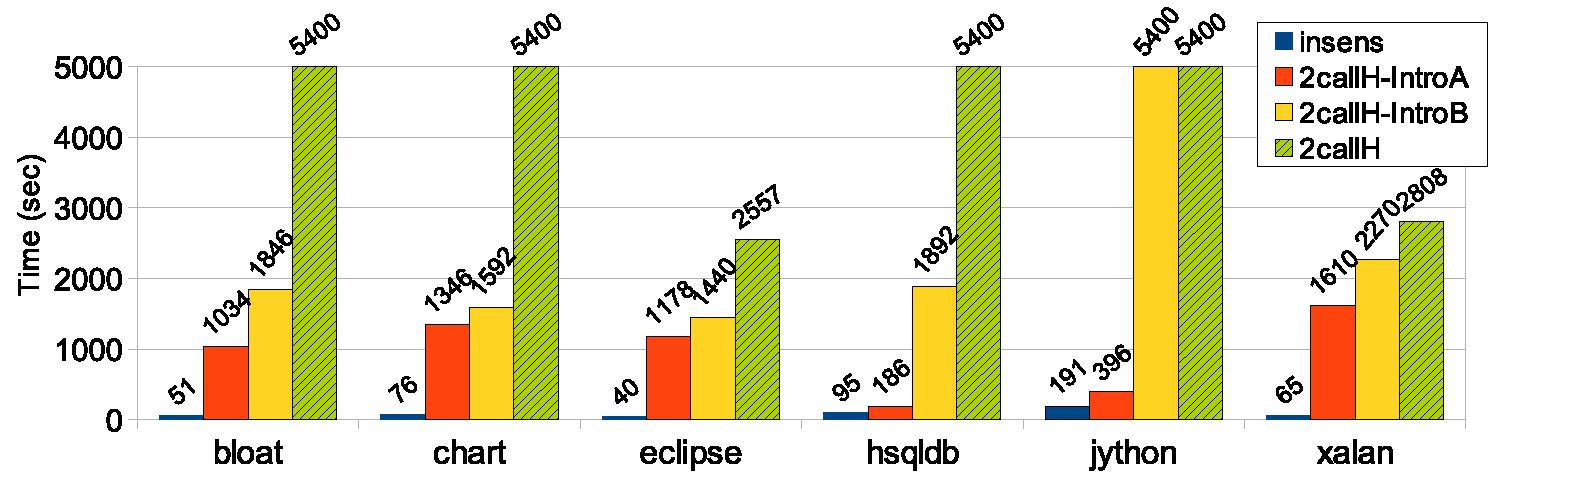
\includegraphics[scale=0.54]{assets/introspective/2callHtime.pdf} \\
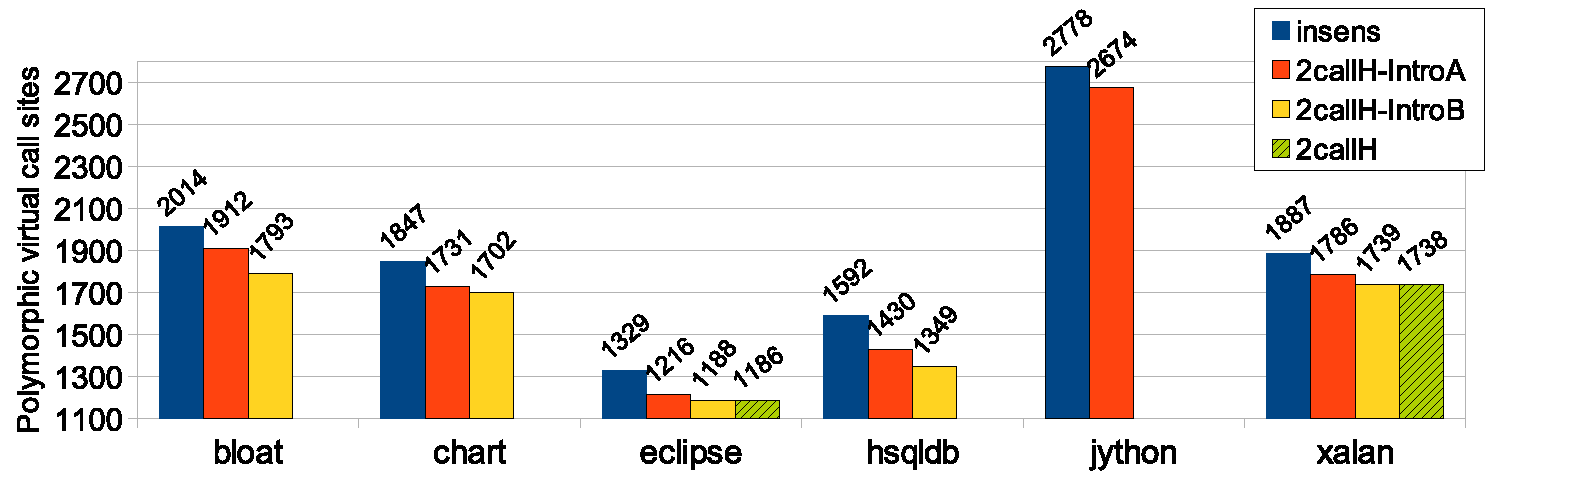
\includegraphics[scale=0.54]{assets/introspective/2callHvcalls.pdf} \\
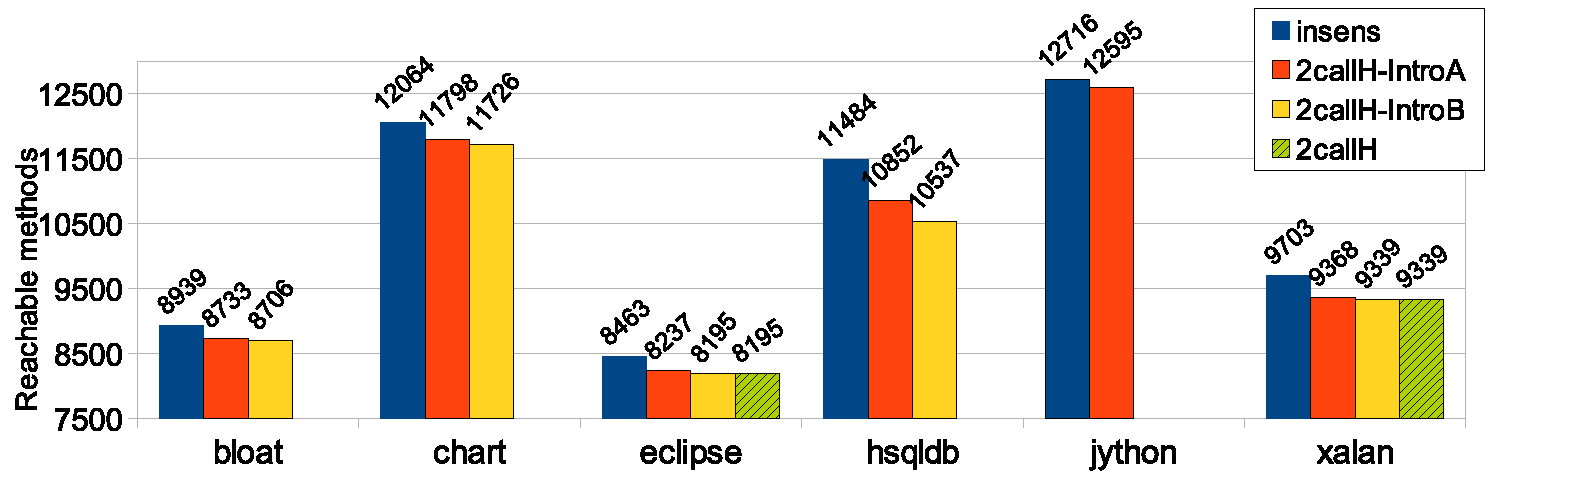
\includegraphics[scale=0.54]{assets/introspective/2callHmeths.pdf} \\
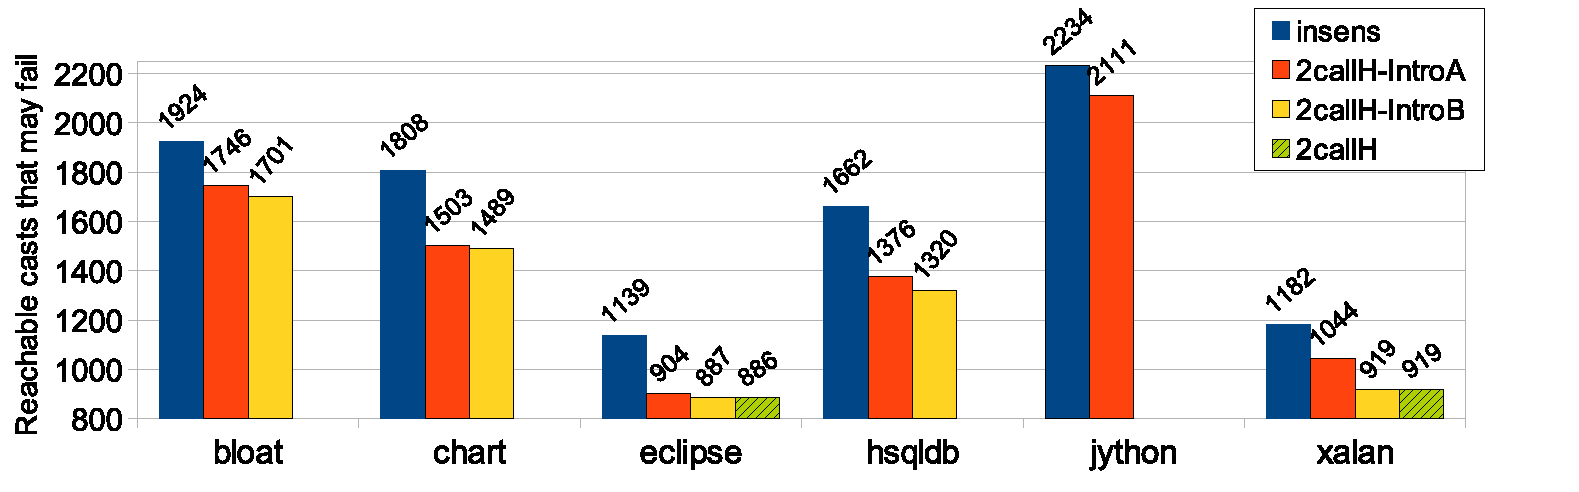
\includegraphics[scale=0.54]{assets/introspective/2callHcasts.pdf}
\end{center}
\caption{Performance and precision (3 separate metrics: calls that cannot be devirtualized, reachable methods, casts that cannot be eliminated) for introspective context-sensitive variants of a \textbf{2callH} analysis, compared with baselines (2callH and insensitive).}
\label{fig:introspect:2callH-chart}
\end{figure*}


The results of our experiments are shown in Figures~\ref{fig:introspect:2objH-chart}, \ref{fig:introspect:2typeH-chart}, and \ref{fig:introspect:2callH-chart}. We evaluate two variants of introspective context-sensitivity corresponding to \emph{Heuristic-A} and \emph{Heuristic-B} from Section~\ref{sec:introspect:heuristics}. We test the three main flavors of context-sensitivity: object-sensitivity \cite{issta:2002:Milanova,article:2005:Milanova}, call-site sensitivity \cite{col:1981:Sharir,thesis:Shivers}, and type-sensitivity~\cite{popl:2011:Smaragdakis}. The three flavors have very different profiles of practical use and scalability, as detailed next.


\subsection{Object-sensitivity}
Deep-context object-sensitive analyses are the most precise in practice, but do not always scale well. Starting from a 2-object-sensitive analysis with a 1-context-sensitive heap (2objH), we define our two introspective versions (2objH-IntroA and 2objH-IntroB for Heuristic-A and Heuristic-B, respectively). Figure~\ref{fig:introspect:2objH-chart} plots first the execution time and then three precision metrics for all analyses. In all cases \emph{lower is better}. There is no real ``metric'' for precision, since each client may have unique needs, but our three metrics together should yield a reasonable projection of precision. Note that since there is no ``ground truth'' for the ideal value of precision metrics, their chart scales are arbitrary (and differences are not as visually pronounced as could be because of plotting multiple benchmarks on a single chart) but the insensitive/2objH analyses serve as upper/lower reference markers in practice. We use a 90min timeout. The jython and hsqldb benchmarks did not terminate for 2objH, and jython did not terminate for 2objH-IntroB either. We indicate non-termination with full bars in the top (time) chart and the absence of bars in the bottom three (precision) charts.

As can be seen in Figure~\ref{fig:introspect:2objH-chart}, the two introspective variants scale much better than the full 2objH analysis. Indeed, IntroA scales to all benchmarks, while showing significant precision gains over an insensitive analysis. IntroB is even more precise: it covers \emph{more than two-thirds} of the precision advantage of 2objH over an insensitive analysis for most benchmarks and precision metrics, while scaling significantly better.


\subsection{Type-sensitivity}
Type-sensitivity is designed with the explicit purpose of providing more scalability than object-sensitivity but in a very different manner: instead of avoiding high context depths, type-sensitivity makes each context element coarser. Thus it is doubly interesting to see if introspection can add benefit to type-sensitive analyses. Type-sensitivity is not immune to the pathologies of object-sensitivity: for instance, in our benchmark set it does not scale to jython. 

Figure~\ref{fig:introspect:2typeH-chart} shows our results, plotting variants of a 2-type-sensitive analysis with a 1-context-sensitive heap (2typeH), and following the same conventions as earlier. (The insensitive baseline is inherited and not re-run.) As can be seen, the IntroB version scales to all programs while typically maintaining very good precision---often close to the full 2typeH. The IntroA version has the desirable feature of near-perfect scalability: its maximum runtime for \emph{any} benchmark is 360sec. At the same time it exhibits precision gains compared to a context-insensitive analysis, although these are noticeably lower than the precision gains of IntroB.


\subsection{Call-site sensitivity}
Call-site sensitivity is the traditional flavor of context-sensitivity---a virtual synonym for the term. In practice, call-site sensitivity is quite good for some analysis clients but almost never scalable at context depths greater than 1. 

As Figure~\ref{fig:introspect:2callH-chart} shows, introspective context-sensitivity performs remarkably well when applied to a 2-call-site-sensitive analysis with a 1-context-sensitive heap (2callH). The base 2callH analysis does not terminate for 4 out of 6 of our benchmarks, while introspective analyses terminate either for all (IntroA) or for nearly all (5 out of 6 for IntroB). Furthermore, IntroB seems to achieve the full precision of 2callH for the two benchmarks for which the latter yields results, and for all different metrics! Combined with the across-the-board scalability gains shown in the timing chart, this confirms the effectiveness of introspection for tuning out extreme analysis costs. IntroA is not far behind in precision, obtaining more than two-thirds of the precision gains of IntroB for most metrics and benchmarks.


\subsection{Discussion}
The above timings of introspective context-sensitivity do not include the cost of first running a context-insensitive analysis, and other timing overheads (relatively constant at about 100sec) related to computing the objects and sites to refine and re-running an analysis.\footnote{Our current implementation has to export facts to disk and re-import them back in memory, as well as regenerate a program representation in order to re-run an analysis.} We did not include these numbers in the timings in order to keep the presentation simpler but also because
\begin{inparaenum}[(a)]
\item our emphasis is on scalability and not on small-scale speed gains---we consider small differences in timings, e.g., in the chart and eclipse benchmarks of Figure~\ref{fig:introspect:2objH-chart}, to be negligible for our purposes; and
\item these constant overheads can be factored out---e.g., with minor engineering we could have incurred them only once per benchmark and not once per run of every introspective analysis variation.
\end{inparaenum}

Based on our experimental results, introspective context-sensitivity achieves its goal: it offers a knob for users to select points in the scalability/precision spectrum. The tradeoffs of cost and precision exhibited by Heuristic-A and Heuristic-B are illustrative. Not only do these heuristics yield different options (more precision vs. more scalability) but they are also very consistent in their tradeoff, throughout multiple benchmarks and analysis flavors.

Finally, note that we used identical introspection heuristics (Heuristic-A and Heuristic-B) with the same constants (see Section~\ref{sec:introspect:heuristics}) for all three context-sensitivity flavors and for all benchmarks. This suggests that there are significant opportunities for further tuning: different heuristics can be used, the constants can be optimized, the constants or the heuristics can be adapted per-benchmark or per-context flavor. However, the goal of our experiments is not to squeeze out a few percentage points of speedup but to show that the simple idea of introspective context-sensitivity can easily offer very useful tradeoffs in scalability and precision.


\section{Summary}

We introduced introspective context-sensitivity: an approach to making context-sensitive analyses scale. The approach consists of defining an analysis with two separate kinds of context. Each program element is analyzed with one kind, selected based on external input. Then, by first running an inexpensive context-insensitive analysis, we can identify program elements that should be treated with a more precise context and others that should be treated less precisely to avoid an explosion in complexity. Our technique applies to any kind of context abstraction and yields scalability \emph{\`{a} la carte}: the user can select a scalability profile and achieve it for a price in precision. As shown in our experiments, this price is not too steep. The precision loss of introspective context-sensitivity can be minuscule (as is for call-site-sensitive analyses), while the scalability gain is substantial.

We believe that introspective context-sensitivity is a big step forward in pointer analysis. It is not just an effective technique, but an effective technique that addresses the major current pain point in practical applications of points-to analyses.